\begin{lstlisting}
Section 6.3: 6, 7,11,16,19
Section 6.4: 2, 3, 5, 6
\end{lstlisting}
\begin{exercise}
\begin{figure}[H]
\centering
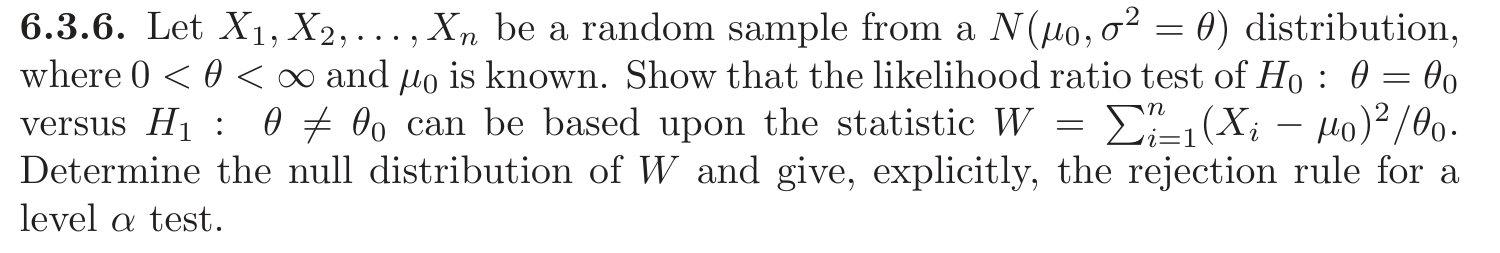
\includegraphics[width=\textwidth]{1-hw9-2025050423.png}
% \caption{}
\label{}
\end{figure}
\end{exercise}
\[
L(\theta)=\prod_{i=1}^{n} f(X_i;\theta)=\prod_{i=1}^{n} \frac{1}{\sqrt{ 2\pi\theta }}e^{ -(X_i-\mu_0)^2/(2\theta) }=(2\pi\theta)^{-n/2}\exp \left\{  -\sum_{i=1}^{n} (X_i-\mu_0)^2/(2\theta)  \right\}
\]
\[
l(\theta)=-\frac{n}{2}\log(2\pi\theta)-\sum_{i=1}^{n} (X_i-\mu_0)^2/(2\theta)
\]
\[
\frac{ \partial l(\theta) }{ \partial \theta } =-\frac{n}{2}\frac{1}{\theta}+\frac{1}{2}\sum_{i=1}^{n} \frac{(X_i-\mu_0)^2}{\theta^{2}}=0\implies \widehat{\theta}=\frac{1}{n}\sum_{i=1}^{n} (X_i-\mu_0)^2
\]
\[
\Lambda=\frac{L(\theta_0)}{L(\widehat{\theta})}=\frac{(2\pi \theta_0)^{-n/2 }\exp \left\{  -\frac{1}{2}W  \right\}}{\left( \frac{2\pi}{n}\sum_{i=1}^{n}(X_i-\mu_0)^2  \right)^{-n/2}\exp \left\{  -\frac{n}{2}  \right\}}=\frac{e^{ -W/2  }}{\left( \frac{W}{n} \right)^{-n/2 }e^{ -n/2 }}=n^{-\frac{n}{2}}W^{\frac{n}{2}}e^{ (n-W)/2 }
\]
Then
\[
-2\log\Lambda=-2\left( -\frac{n}{2}\log n+\frac{n}{2}\log W+\frac{n-W}{2} \right)\sim \chi^{2}(1)
\]
We reject $H_0$ at level $\alpha$ when
\begin{equation}
-n\log n-n-n\log W+W\in(0,\chi^{2}_{\alpha/2 }(1)]\cup[\chi^{2}_{1-\alpha/2 }(1),\infty)
\label{49c1a0}
\end{equation}

\begin{remark}
Here we use $(0,\chi^{2}_{\alpha/2 }(1)]\cup[\chi^{2}_{1-\alpha/2 }(1),\infty)$ instead of $[\chi^{2}_{\alpha}(1),\infty)$, just for fun.
\end{remark}
\begin{exercise}
\begin{figure}[H]
\centering
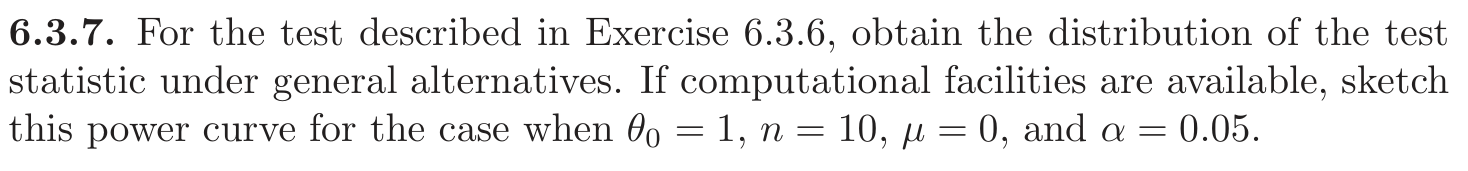
\includegraphics[width=\textwidth]{2-hw9-2025050423.png}
% \caption{}
\label{}
\end{figure}
\end{exercise}
Under the general alternatives,
\[
W=\frac{\theta}{\theta_0}\sum_{i=1}^{n} \left( \frac{X_i-\mu_0}{\sqrt{ \theta }} \right)^2
\]
\[
\frac{X_i-\mu_0}{\sqrt{ \theta }}\sim N(0,1)\Rightarrow\left( \frac{X_i-\mu_0}{\sqrt{ \theta }} \right)^2 \sim \chi^{2}(1)
\]
Thus
\[
\frac{\theta_0}{\theta}W\sim \chi^{2}(n)
\]
\[
\begin{aligned}
f_{W}(x) & =\frac{ \partial   }{ \partial x } \mathbb{P}(W\leq x) \\
 & =\frac{ \partial   }{ \partial x } \mathbb{P}\left( \frac{\theta_0}{\theta}W\leq \frac{\theta_0}{\theta}x \right) \\
 & =\frac{\theta_0}{\theta}f_{\chi^{2}(n)}\left( \frac{\theta_0}{\theta}x \right) \\
 & =\frac{\theta_0}{\theta}\cdot\frac{1}{\Gamma(n/2 )2^{n/2 }}\left( \frac{\theta_0}{\theta}x \right)^{n/2-1 }e^{ -\theta_0x/(2\theta) } \\
 & =\frac{1}{\Gamma(n/2 )(2\theta/\theta_0)^{n/2 }}x^{n/2-1}e^{ -x/(2\theta/\theta_0) }
\end{aligned}
\]
Therefore
\[
W\sim \Gamma\left( \frac{n}{2},\frac{2\theta}{\theta_0} \right)
\]
\begin{lstlisting}[language=mathematica]
(* 设置参数 *)
alpha = 0.05;
n = 10;

(* 定义您的方程表达式 *)
equation = -n Log[n] - n - n Log[W] + W;

(* 计算所需的分布分位数 *)
lowerQuantile = Quantile[ChiSquareDistribution[1], alpha/2];
upperQuantile = Quantile[ChiSquareDistribution[1], 1 - alpha/2];

(* 联立两个不等式并求解 W *)
Reduce[
    (equation <= lowerQuantile) && (equation >= upperQuantile),
    W
]
\end{lstlisting}
Solve \cref{49c1a0} , we get
\[
0.0369204\leq W\leq 76.3847\lor 0<W\leq 0.0223095\lor W\geq 82.1332
\]
i.e.
\[
\sum_{i=1}^{n} X_i^2\in(0,0.0223095]\cup[0.0369204,76.3847]\cup[82.1332,\infty)
\]
\begin{exercise}
\begin{figure}[H]
\centering
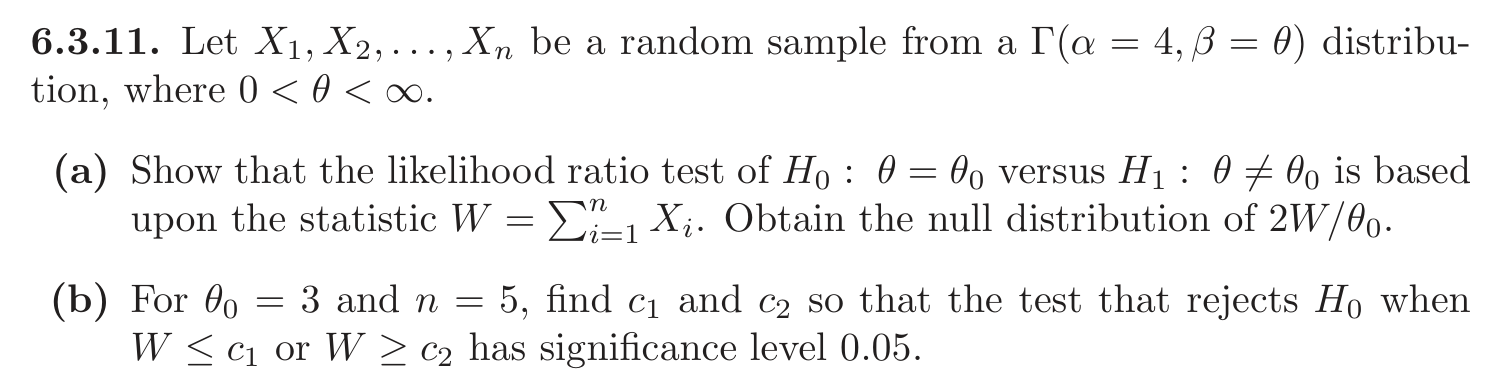
\includegraphics[width=\textwidth]{3-hw9-2025050423.png}
% \caption{}
\label{}
\end{figure}
\end{exercise}
(a)
\[
L(\theta)=\prod_{i=1}^{n} \frac{1}{\Gamma(4)\theta^{4}}X_i^{3}e^{ -X_i/\theta }=\prod_{i=1}^{n} \frac{1}{6\theta^{4}}X_i^{3}e^{ -X_i/\theta }=\frac{1}{6^{n}\theta^{4n}}\left( \prod_{i=1}^{n} X_i \right)^{3}\exp \left\{  -\frac{1}{\theta}\sum_{i=1}^{n} X_i  \right\}
\]
\[
l(\theta)=-\log(6^{n})-4n\log\theta+3\sum_{i=1}^{n} \log X_i-\frac{1}{\theta}\sum_{i=1}^{n} X_i
\]
\[
\frac{ \partial l(\theta) }{ \partial \theta } =-\frac{4n}{\theta}+\frac{1}{\theta^{2}}\sum_{i=1}^{n} X_i=0\implies\widehat{\theta}=\frac{1}{4n}\sum_{i=1}^{n} X_i
$$ $$
\begin{aligned}
\lambda & =2\log\left( \frac{L(\widehat{\theta})}{L(\theta_0)} \right)=2\log\left( \frac{\theta_0^{4n}}{\left( \frac{1}{4n}\sum_{i=1}^{n}X_i  \right)^{4n}}\exp \left\{  \frac{1}{\theta_0}\sum_{i=1}^{n} X_i-4n  \right\} \right) \\
 & =\frac{2}{\theta_0}\sum_{i=1}^{n} X_i-8n +8n\log\theta_0 -8n\log\left( \frac{1}{4n}\sum_{i=1}^{n} X_i \right) \\
 & =\frac{2}{\theta_0}W-8n\log W-8n+8n\log\theta_0 +8n\log(4n) \\
 & \sim \chi^{2}(1)
\end{aligned}
\]
To obtain the null distribution of $2W/\theta_0$, we first have $W\sim \Gamma(4n,\theta_0)$. Then
\[
\begin{aligned}
f_{2W/\theta_0}(x) & =\frac{ \partial   }{ \partial x } \mathbb{P}(2W/\theta_0\leq x) \\
 & =\frac{\theta_0}{2}\frac{ \partial   }{ \partial x } \mathbb{P}(W\leq x\theta_0/2 ) \\
 & =\frac{\theta_0}{2}f_{W}\left( \frac{\theta_0x}{2} \right) \\
 & =\frac{\theta_0}{2}\frac{1}{6\theta_0^{4}} \left( \frac{\theta_0x}{2} \right)^{3}e^{ -x/2 } \\
 & =\frac{x^{3}}{96}e^{ -x/2  }
\end{aligned}
\]
(b)

\begin{lstlisting}[language=mathematica]
\[Theta]0 = 3; 
n = 5;
alpha = 0.05;
Reduce[2/\[Theta]0  W - 8  n  Log[W] - 8  n + 8  n  Log[\[Theta]0] + 
   8  n  Log[4  n] >= Quantile[ChiSquareDistribution[1], 1 - alpha], W]
\end{lstlisting}
\[
0<W\leq 37.3971\lor W\geq 90.2695
\]
Then $c_1=37.3971,c_2=90.2695$.

\begin{exercise}
\begin{figure}[H]
\centering
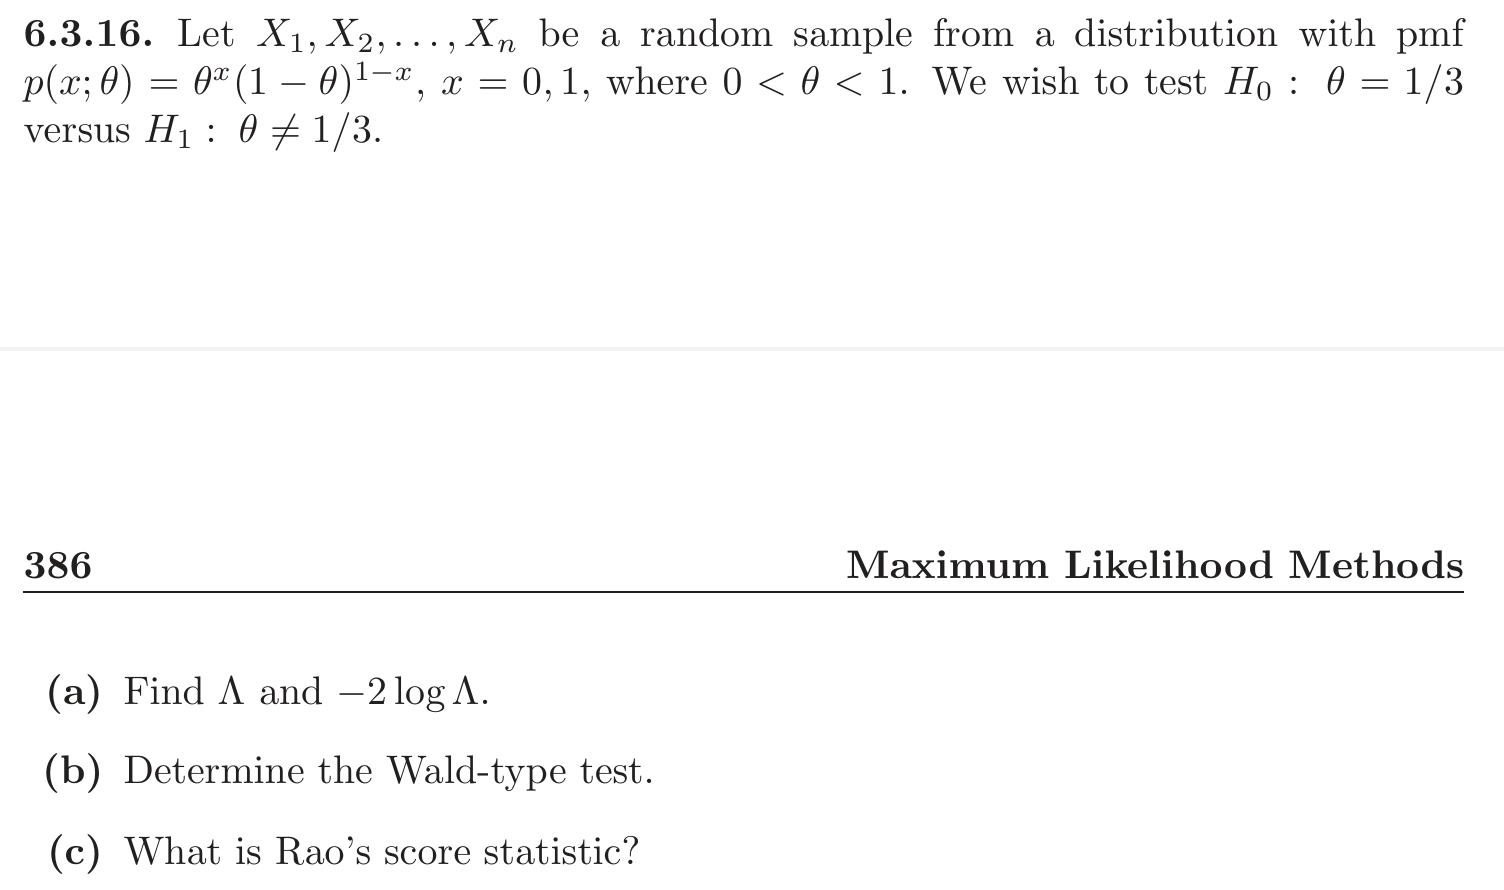
\includegraphics[width=\textwidth]{4-hw9-2025050423.png}
% \caption{}
\label{}
\end{figure}
\end{exercise}
(a)
\[
L(\theta)=\prod_{i=1}^{n} p(X_i;\theta)=\prod_{i=1}^{n} \theta^{X_i}(1-\theta)^{1-X_i}=\theta^{\sum_{i=1}^{n} X_i}(1-\theta)^{n-\sum_{i=1}^{n} X_i}
\]
\[
l(\theta)=\left( \sum_{i=1}^{n} X_i \right)\log\theta+\left( n-\sum_{i=1}^{n} X_i \right)\log(1-\theta)
\]
\[
\begin{aligned}
\frac{ \partial l(\theta) }{ \partial \theta }  & =\frac{1}{\theta}\sum_{i=1}^{n} X_i-\frac{1}{1-\theta}\left( n-\sum_{i=1}^{n} X_i \right) \\
 & =\frac{1}{\theta(1-\theta)}\left[ (1-\theta)\sum_{i=1}^{n} X_i-\theta\left( n-\sum_{i=1}^{n} X_i  \right) \right] \\
 & =\frac{1}{\theta(1-\theta)}\left[ \sum_{i=1}^{n} X_i-\theta n \right]
\end{aligned}
\]
Let $\frac{ \partial l(\theta) }{ \partial \theta }=0$ then we have the solution $\widehat{\theta}=\frac{1}{n}\sum_{i=1}^{n}X_i$. Since $\theta_0=\frac{1}{3}$, denote $W=\sum_{i=1}^{n}X_i$
\[
\begin{aligned}
\Lambda & =\frac{L(\theta_0)}{L(\widehat{\theta})}=\frac{3^{-\sum_{i=1}^{n} X_i}2^{n-\sum_{i=1}^{n}X_i }3^{\sum_{i=1}^{n} X_i-n}}{\left( \frac{1}{n}\sum_{i=1}^{n} X_i \right)^{\sum_{i=1}^{n} X_i}\left( 1-\frac{1}{n}\sum_{i=1}^{n} X_i \right)^{\left( n-\sum_{i=1}^{n} X_i \right)}} \\
 & =\frac{2^{n-\sum_{i=1}^{n}X_i }\cdot 3^{-n}}{\left( \frac{1}{n}\sum_{i=1}^{n} X_i \right)^{\sum_{i=1}^{n} X_i}\left( 1-\frac{1}{n}\sum_{i=1}^{n} X_i \right)^{\left( n-\sum_{i=1}^{n} X_i \right)}} \\
 & =\frac{2^{n-W}\cdot3^{-n}}{\left( \frac{1}{n}W \right)^{W}\left( 1-\frac{1}{n}W \right)^{n-W}}
\end{aligned}
\]
\[
\begin{aligned}
-2\log\Lambda & =(-2)\left[ \log(2^{n-W}\cdot3^{-n})-\log\left( \left( \frac{1}{n}W \right)^{W}\cdot\left( 1-\frac{1}{n}W \right)^{n-W} \right) \right] \\
 & =2(W-n)\log2+2n\log3+2W\log W-2W\log n+2(n-W)\log(n-W)-2(n-W)\log n \\
 & =2(W-n)\log2+2n\log3+2W\log W+2(n-W)\log(n-W)-2n\log n
\end{aligned}
\]
(b)
\[
\begin{aligned}
\frac{ \partial \log p(X;\theta) }{ \partial x }  & =\frac{ \partial   }{ \partial \theta } \log(\theta^{X}(1-\theta )^{1-X}) \\
 & =\frac{ \partial   }{ \partial \theta } (X\log\theta+(1-X)\log(1-\theta)) \\
 & =\frac{X}{\theta}-\frac{1-X}{1-\theta}
\end{aligned}
\]
\[
\frac{ \partial^2 \log p(X;\theta) }{ \partial \theta ^2 }=-\frac{X}{\theta^{2}}-\frac{1-X}{(1-\theta)^2}
\]
\[
\mathbb{E}[X]=\theta
\]
\[
\begin{aligned}
I(\theta) & =\mathbb{E}\left[ -\frac{ \partial^2 \log p(X;\theta) }{ \partial \theta ^2 }  \right]=\mathbb{E}\left[ \frac{X}{\theta^{2}}+\frac{1-X}{(1-\theta )^2} \right] \\
 & =\frac{1}{\theta^{2}}\mathbb{E}[X]+\frac{1}{(1-\theta)^2}\mathbb{E}[1-X] \\
 & =\frac{1}{\theta}+\frac{1}{1-\theta} \\
 & =\frac{1}{\theta(1-\theta)}
\end{aligned}
\]
\[
\begin{aligned}
\chi^{2}_{W} & =\{ \sqrt{ nI(\widehat{\theta}) }(\widehat{\theta}-\theta_0) \}^{2}=nI(\widehat{\theta})\cdot(\widehat{\theta}-\theta_0)^2  \\
 & =n\cdot\frac{1}{\widehat{\theta}(1-\widehat{\theta})}\cdot(\widehat{\theta}-\theta_0)^2 \\
 & =n\cdot\frac{1}{\frac{1}{n}W\left( 1-\frac{1}{n}W \right)}\cdot\left( \frac{1}{n}W-\frac{1}{3} \right)^2 \\
 & =\frac{n}{W(n-W)}\left( W-\frac{n}{3} \right)^2
\end{aligned}
\]
The Wald-test is
\[
\text { Reject } H_0 \text { in favor of } H_1 \text { if } \chi_W^2 \geq \chi_\alpha^2(1) \text {. }
\]
(c)
\[
l'(\theta)=\sum_{i=1}^{n} \frac{ \partial \log p(X_i;\theta) }{ \partial \theta } =\sum_{i=1}^{n} \left( \frac{X_i}{\theta}-\frac{1-X_i}{1-\theta} \right)=\frac{1}{\theta(1-\theta)}\sum_{i=1}^{n} X_i-\frac{n}{1-\theta}
\]
The Rao's score statistic is
\[
\begin{aligned}
\chi^{2}_{R} & =\left( \frac{l'(\theta_0)}{\sqrt{ nI(\theta_0) }} \right)^2 \\
 & =\frac{\left[ \frac{1}{\theta_0 (1-\theta_0)}\sum_{i=1}^{n} X_i-\frac{n}{1-\theta_0} \right]^2}{nI(\theta_0)} \\
 & =\frac{\left[\frac{9}{2}\sum_{i=1}^{n} X_i-\frac{3}{2}n \right]^2}{\frac{9}{2}n}
\end{aligned}
\]
\begin{exercise}
\begin{figure}[H]
\centering
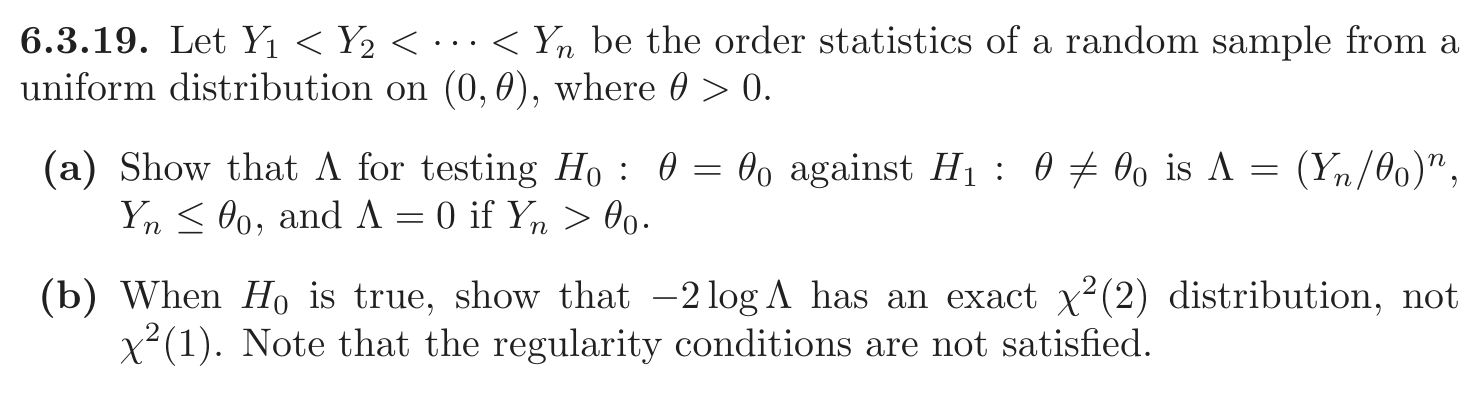
\includegraphics[width=\textwidth]{5-hw9-2025050423.png}
% \caption{}
\label{}
\end{figure}
\end{exercise}
(a)
\[
L(\theta)=\prod_{i=1}^{n} f(X_j;\theta)=\frac{1}{\theta^{n}}\mathbf{1}_{X_{(1)}>0}\mathbf{1}_{X_{(n)}<\theta}
\]
where $X_{(1)}=\min\{ X_1,\dots,X_n \}$ and $X_{(n)}=\max\{ X_1,\dots,X_n \}$. Assuming all $X_i>0$, then
\[
L(\theta)=\frac{1}{\theta^{n}}\mathbf{1}_{\theta\geq Y_n}
\]
Then
\[
\Lambda=\frac{\sup_{\theta\in\Theta_0}L(\theta)}{\sup_{\theta\in\Theta}L(\theta)}=\frac{1}{\theta^{n}_{0}}\cdot Y_n^{n}\cdot \mathbf{1}_{\theta_0\geq Y_n}
\]
(b)
When $H_0$ is true, we have
\[
-2\log\Lambda=-2n\log\frac{Y_n}{\theta_0}\cdot \mathbf{1}_{\theta_0\geq Y_n}
\]
\[
f_{Y_n}(x)=\frac{x^{n-1}}{(n-1)!}\cdot n!\cdot\frac{1}{\theta^{n}}=\frac{n}{\theta^{n}}x^{n-1}
\]
Then
\[
\begin{aligned}
\mathbb{P}(-2\log\Lambda\leq x) & =\mathbb{P}(\Lambda\geq e^{ -x/2  })=\mathbb{P}\left( Y_n\geq \theta_0e^{ -\frac{x}{2n} } \right) \\
 & =1-\mathbb{P}\left( Y_n<\theta_0e^{ -\frac{x}{2n} } \right) \\
 & =1-\mathbb{P}\left( X_j<\theta_0e^{ -\frac{x}{2n} };\forall j \right) \\
 & =1-\left( \frac{\theta_0e^{ -\frac{x}{2n} }}{\theta_0} \right)^{n} \\
 & =1-e^{ -\frac{x}{2} } 
\end{aligned}
\]
Thus
\[
f_{-2\log\Lambda}(x)=\frac{ \partial   }{ \partial x } \mathbb{P}(-2\log\Lambda\leq x)=\frac{1}{2}e^{ -\frac{x}{2} }
\]
Hence $-2\log\Lambda \sim \chi^{2}(2)$.

\begin{exercise}
\begin{figure}[H]
\centering
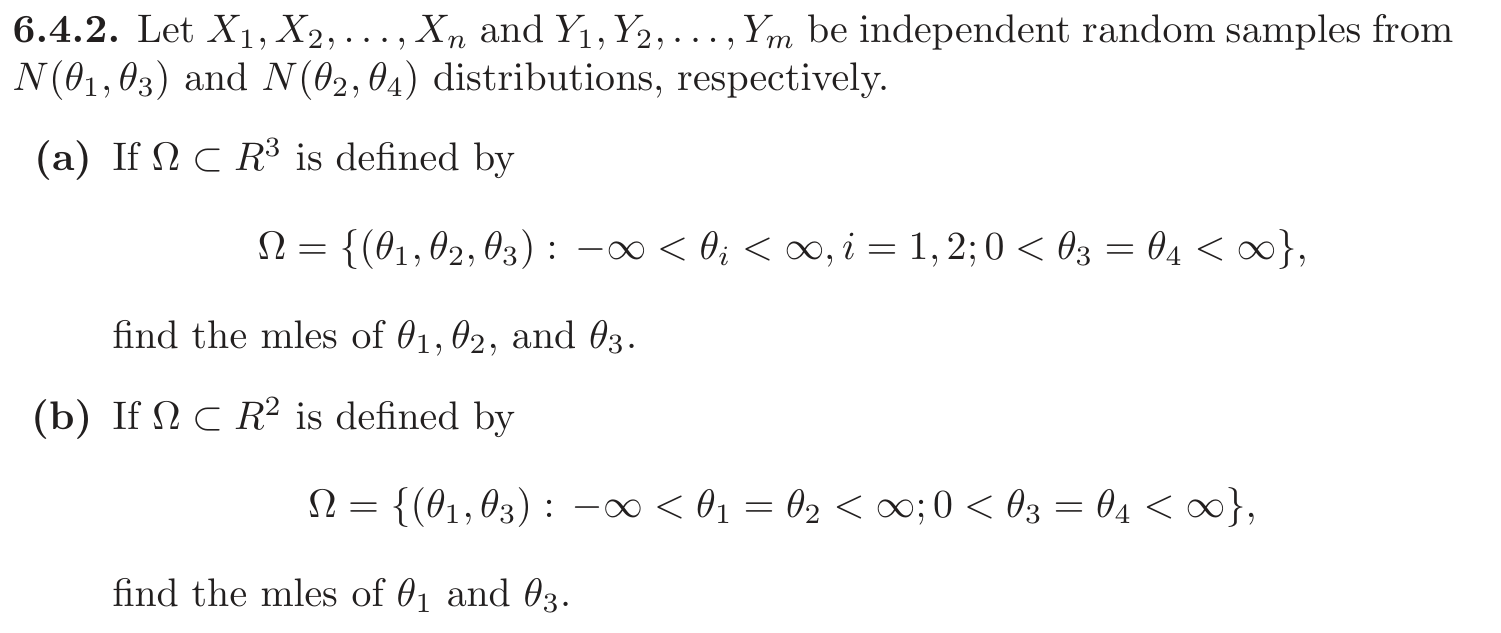
\includegraphics[width=\textwidth]{6-hw9-2025050423.png}
% \caption{}
\label{}
\end{figure}
\end{exercise}
(a)
Let $\boldsymbol{\theta}=(\theta_1,\theta_2,\theta_3)\in \Omega$, then
\[
\begin{aligned}
L(\boldsymbol{\theta}) & =\prod_{i=1}^{n} f_{X}(X_i;\theta_1,\theta_3)\cdot f_{Y}(Y_i;\theta_2,\underbrace{ \theta_4 }_{ =\theta_3 }) \\
 & =\prod_{i=1}^{n} \frac{1}{\sqrt{ 2\pi\theta_3 }}e^{ -(X_i-\theta_1)^2/(2\theta_3) }\cdot\frac{1}{\sqrt{ 2\pi\theta_3 }}e^{ -(Y_i-\theta_2)^2/(2\theta_3) } \\
 & =(2\pi\theta_3)^{-n}\exp \left\{ - \sum_{i=1}^{n} \frac{(X_i-\theta_1)^2+(Y_i-\theta_2)^2}{2\theta_3}  \right\}
\end{aligned}
\]
\[
l(\boldsymbol{\theta})=-n\log(2\pi\theta_3)-\sum_{i=1}^{n} \frac{(X_i-\theta_1)^2+(Y_i-\theta_2)^2}{2\theta_3}
\]
\[
\frac{ \partial   }{ \partial \boldsymbol{\theta} } l(\boldsymbol{\theta})=\left( \frac{1}{\theta_3}\sum_{i=1}^{n} (X_i-\theta_1),\frac{1}{\theta_3}\sum_{i=1}^{n}(Y_i-\theta_2),-\frac{n}{\theta_3}+\frac{1}{2\theta_3^2}\sum_{i=1}^{n} [(X_i-\theta_1)^2+(Y_i-\theta_2)^2]  \right)
\]
Let $\frac{ \partial  }{ \partial \boldsymbol{\theta} }l(\boldsymbol{\theta})=0$, then the mles of $\theta_1$, $\theta_2$ and $\theta_3$ are
\[
\widehat{\theta}_1=\frac{1}{n}\sum_{i=1}^{n} X_i,\quad \widehat{\theta}_2=\frac{1}{n}\sum_{i=1}^{n} Y_i,\quad \widehat{\theta}_3=\frac{1}{2n}\left( \sum_{i=1}^{n} (X_i^2+Y_i^2)-\frac{1}{n}\left( \sum_{i=1}^{n} X_i \right)^2-\frac{1}{n}\left( \sum_{i=1}^{n} Y_i \right)^2 \right)
\]
(b)
\[
l(\boldsymbol{\theta})=-n\log(2\pi\theta_3)-\sum_{i=1}^{n} \frac{(X_i-\theta_1)^2+(Y_i-\theta_1)^2}{2\theta_3}
\]
\[
\frac{ \partial l(\boldsymbol{\theta}) }{ \partial \boldsymbol{\theta} } =\left( \frac{1}{\theta_3}\sum_{i=1}^{n} (X_i+Y_i-2\theta_1),-\frac{n}{\theta_3}+\frac{1}{2\theta_3^2}\sum_{i=1}^{n} [(X_i-\theta_1)^2+(Y_i-\theta_1)^2] \right)
\]
Let $\frac{ \partial  }{ \partial \boldsymbol{\theta} }l(\boldsymbol{\theta})=0$, then the mles of $\theta_1$ and $\theta_3$ are
\[
\widehat{\theta}_{1}=\frac{1}{2n}\sum_{i=1}^{n} (X_i+Y_i)\qquad \widehat{\theta}_3=\frac{1}{2n}\left( \sum_{i=1}^{n} (X_i^2+Y_i^2)-\frac{1}{n}\left( \sum_{i=1}^{n} X_i \right)^2-\frac{1}{n}\left( \sum_{i=1}^{n} Y_i \right)^2 \right)
\]
\begin{exercise}
\begin{figure}[H]
\centering
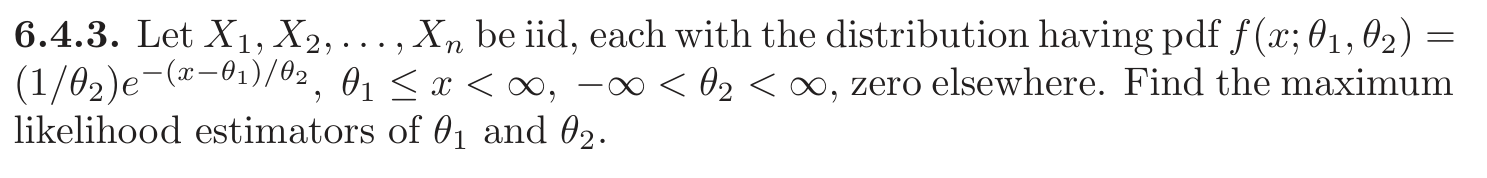
\includegraphics[width=\textwidth]{7-hw9-2025050423.png}
% \caption{}
\label{}
\end{figure}
\end{exercise}
\[
L(\boldsymbol{\theta})=\prod_{i=1}^{n} f(X_i;\theta_1,\theta_2)=\prod_{i=1}^{n}\theta_2^{-1}\exp \left\{  -\frac{X_i-\theta_1}{\theta_2}  \right\}=\theta_2^{-n}\exp \left\{  -\frac{1}{\theta_2}\sum_{i=1}^{n} X_i+\frac{n\theta_1}{\theta_2}  \right\}
\]
\[
l(\boldsymbol{\theta})=-n\log\theta_2-\frac{1}{\theta_2}\sum_{i=1}^{n} X_i+\frac{n\theta_1}{\theta_2}
\]
\[
\frac{ \partial l(\boldsymbol{\theta}) }{ \partial \theta_2 } =-\frac{n}{\theta_2}+\frac{1}{\theta_2^2}\sum_{i=1}^{n} X_i-\frac{n\theta_1}{\theta_2^2}
\]
The mles of $\theta_1$ and $\theta_2$ are
\[
\widehat{\theta}_{1}=\min\{ X_1,\dots,X_n \},\qquad \widehat{\theta}_{2}=\frac{1}{n}\sum_{i=1}^{n} X_i-\widehat{\theta}_{1}=\frac{1}{n}\sum_{i=1}^{n} X_i-\min\{ X_1,\dots,X_n \}
\]
\begin{exercise}
\begin{figure}[H]
\centering
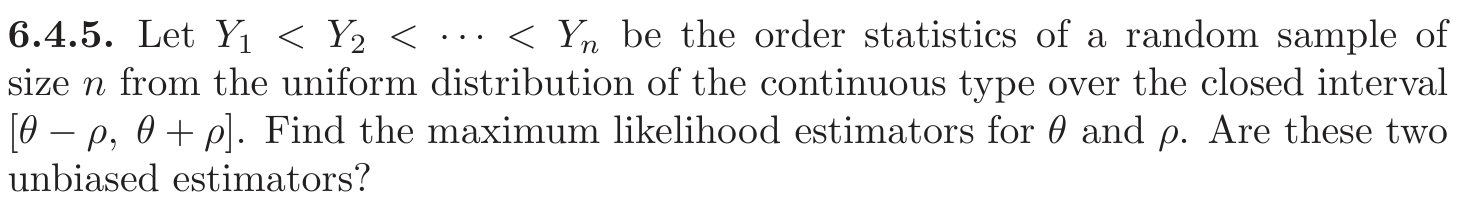
\includegraphics[width=\textwidth]{hw9-2025050500.png}
% \caption{}
\label{}
\end{figure}
\end{exercise}
\[
X\sim \text{Unif}[\theta-\rho,\theta+\rho]
\]
\[
L(\theta,\rho)=\prod_{i=1}^{n} \frac{1}{2\rho}\mathbf{1}_{\theta-\rho\leq X_i\leq \theta+\rho}=\frac{1}{(2\rho)^n}\mathbf{1}_{Y_1\geq \theta-\rho}\cdot \mathbf{1}_{Y_n\leq \theta+\rho}
\]
We have $2\rho\geq Y_n-Y_1$, then $L(\theta,\rho)\leq\frac{1}{(Y_n-Y_1)^n}$. The equality holds iff $Y_1=\theta-\rho$, $Y_n=\theta+\rho$.

Thus $\widehat{\theta}=\frac{Y_1+Y_n }{2}$, $\widehat{\rho}=\frac{Y_n-Y_1}{2}$.
\[
\begin{aligned}
f_{Y_1}(x) & =\frac{ \partial  }{ \partial x } \mathbb{P}(Y_1\leq x)=\frac{ \partial   }{ \partial x } (1-\mathbb{P}(Y_1>x)) \\
 & =\frac{ \partial   }{ \partial x } \left( 1-\left( \frac{\theta+\rho-x}{2\rho} \right)^n \right)=\frac{1}{(2\rho)^{n}}\cdot n\cdot(\theta+\rho-x)^{n-1}
\end{aligned}
\]
\[
f_{Y_n }(x)=\frac{ \partial   }{ \partial x } \mathbb{P}(Y_n\leq x)=\frac{ \partial   }{ \partial x } \left( \frac{x-\theta+\rho}{2\rho} \right)^{n}=\frac{1}{( 2\rho)^{n}}\cdot n (x-\theta+\rho)^{n-1}
\]
Then
\[
\begin{aligned}
\mathbb{E}\widehat{\theta} & =\frac{1}{2}(\mathbb{E}Y_1+\mathbb{E}Y_n) \\
 & =\frac{1}{2}\int_{\theta-\rho}^{\theta+\rho} \frac{1}{(2\rho)^{n}} nx(\theta+\rho-x)^{n-1} \, \mathrm{d}x +\frac{1}{2}\int_{\theta-\rho}^{\theta+\rho} \frac{1}{(2\rho)^{n}} nx(x-\theta+\rho)^{n-1} \, \mathrm{d}x \\
 & =\theta
\end{aligned}
\]
\[
\begin{aligned}
\mathbb{E}\widehat{\rho} & =\frac{1}{2}(\mathbb{E}Y_n-\mathbb{E}Y_1) \\
 & =-\frac{1}{2}\int_{\theta-\rho}^{\theta+\rho} \frac{1}{(2\rho)^{n}} nx(\theta+\rho-x)^{n-1} \, \mathrm{d}x +\frac{1}{2}\int_{\theta-\rho}^{\theta+\rho} \frac{1}{(2\rho)^{n}} nx(x-\theta+\rho)^{n-1} \, \mathrm{d}x \\
 & =\frac{(n-1) \rho }{n+1}
\end{aligned}
\]
Therefore, $\widehat{\theta}$ is unbiased, $\widehat{\rho}$ is not unbiased.

\begin{lstlisting}[language=mathematica]
-(1/2)*Integrate[(1/(2*\[Rho])^n)*n*x*(\[Theta] + \[Rho] - x)^(n - 1), {x, \[Theta] - \[Rho], \[Theta] + \[Rho]}] + (1/2)*Integrate[(1/(2*\[Rho])^n)*n*x*(x - \[Theta] + \[Rho])^(n - 1), {x, \[Theta] - \[Rho], \[Theta] + \[Rho]}]
\end{lstlisting}
\begin{exercise}
\begin{figure}[H]
\centering
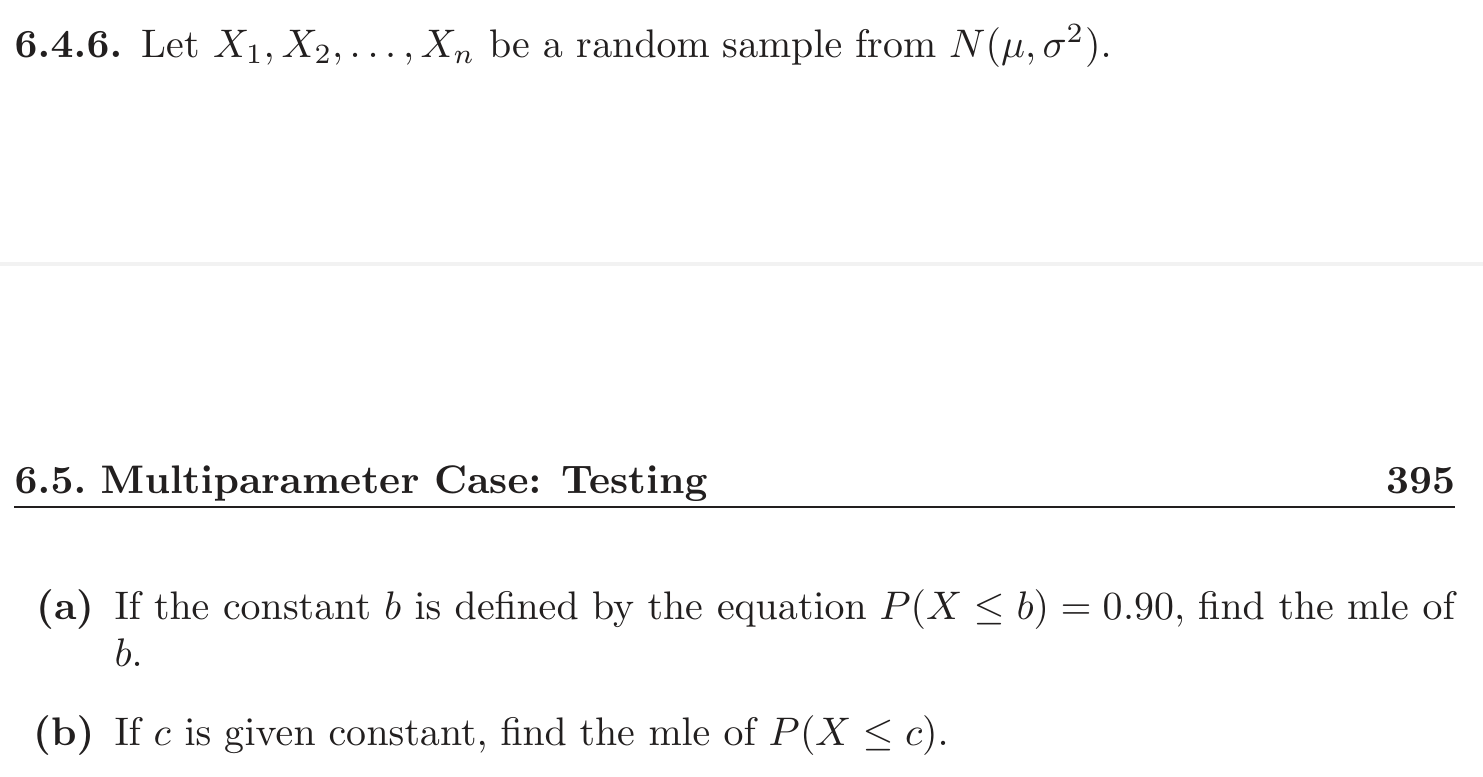
\includegraphics[width=\textwidth]{1-hw9-2025050500.png}
% \caption{}
\label{}
\end{figure}
\end{exercise}
(a)
The mle of $\mu$ and $\sigma^{2}$ are
\[
\widehat{\mu}=\frac{1}{n}\sum_{i=1}^{n} X_i,\quad \widehat{\sigma}^2=\frac{1}{n}\sum_{i=1}^{n} (X_i-\overline{X})^2
\]
Then
\[
\mathbb{P}(X\leq b)=\mathbb{P}\left( \frac{X-\mu}{\sigma}\leq \frac{b-\mu}{\sigma} \right)=0.90
\]
Thus
\[
\frac{b-\mu}{\sigma}=\Phi(0.90)\Rightarrow b=\mu+\sigma \Phi(0.90)\Rightarrow \widehat{b}=\widehat{\mu}+\Phi(0.90)\cdot\widehat{\sigma}
\]
where $\Phi(0.90)\approx1.2816$, thus the mle of $b$ is
\[
\widehat{b}=\frac{1}{n}\sum_{i=1}^{n} X_i+1.2816\cdot \sqrt{ \frac{1}{n}\sum_{i=1}^{n} (X_i-\overline{X})^2 }
\]
(b)
\[
p\coloneqq \mathbb{P}(X\leq c)=\mathbb{P}\left( \frac{X-\mu}{\sigma}\leq \frac{c-\mu}{\sigma} \right)=\Phi\left( \frac{c-\mu}{\sigma} \right)
\]
Thus the mle of $p$ is
\[
\widehat{p}=\Phi\left( \frac{c-\widehat{\mu}}{\widehat{\sigma}} \right)=\Phi\left( \frac{c-\frac{1}{n}\sum_{i=1}^{n} X_i}{\sqrt{ \frac{1}{n}\sum_{i=1}^{n} (X_i-\overline{X})^2 }} \right)
\]